

% Q18
\question The figure shows a right prism. Find the volume of the prism.

\begin{minipage}{0.45\textwidth}
\begin{choices}
    \choice $216\text{ cm}^3$
    \choice $240\text{ cm}^3$
    \correctchoice $300\text{ cm}^3$
    \choice $328\text{ cm}^3$
\end{choices}
\end{minipage}
\begin{minipage}{0.52\textwidth}
\centering
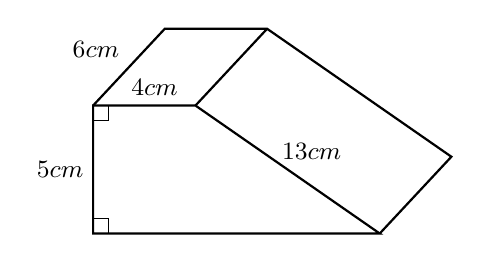
\begin{tikzpicture}[scale=0.65]
    \coordinate (A) at (0,0);
    \coordinate (B) at (0,2.5);
    \coordinate (C) at (2,2.5);
    \coordinate (D) at (5.6,0);
    \coordinate (B') at (1.4,4.0);
    \coordinate (C') at (3.4,4.0);
    \coordinate (D') at (7.0,1.5);
    \draw[thick] (A) -- (B) -- (C) -- (D) -- cycle;
    \draw[thick] (B) -- (B') -- (C') -- (D') -- (D);
    \draw[thick] (C) -- (C');
    \draw (0,2.2) -- (0.3,2.2) -- (0.3,2.5);
    \draw (0,0.3) -- (0.3,0.3) -- (0.3,0);
    \node[left] at (0,1.25) {\small $5\text{ cm}$};
    \node[above] at (1.2,2.5) {\small $4\text{ cm}$};
    \node[above left] at (0.7,3.25) {\small $6\text{ cm}$};
    \node[above right] at (3.5,1.25) {\small $13\text{ cm}$};
\end{tikzpicture}
\end{minipage}
\begin{solution}
The bottom base of the trapezoidal cross-section is $4 + \sqrt{13^2 - 5^2} = 4 + 12 = 16\text{ cm}$. \\
Volume of the prism $= \frac{1}{2}(4 + 16)(5)(6) = 300\text{ cm}^3$ (C).
\end{solution}

% Q19
\question In the figure, $OAB$ and $OCD$ are sectors with centre $O$ , where $OA = 33\text{ cm}$ and $OC = 39\text{ cm}$ . The area of the shaded region $ABDC$ is $72\pi\text{ cm}^2$ . Which of the following is/are true?

\begin{minipage}{0.48\textwidth}
\begin{itemize}
    \item[I.] The angle of the sector $OAB$ is $60^\circ$ .
    \item[II.] The area of the sector $OAB$ is $11\pi\text{ cm}^2$ .
    \item[III.] The perimeter of the sector $OCD$ is $13\pi\text{ cm}$ .
\end{itemize}
\begin{choices}
    \correctchoice I only
    \choice II only
    \choice I and III only
    \choice II and III only
\end{choices}
\end{minipage}
\begin{minipage}{0.48\textwidth}
\centering
\begin{tikzpicture}[scale=0.08]
    \coordinate (O) at (0,0);
    \fill[pattern=north east lines] (-30:33) arc (-30:30:33) -- (30:39) arc (30:-30:39) -- cycle;
    \draw[thick] (O) -- (-30:39) arc (-30:30:39) -- cycle;
    \draw[thick] (-30:33) arc (-30:30:33);
    \node[left] at (O) {$O$};
    \node[below left] at (-30:33) {$A$};
    \node[above left] at (30:33) {$B$};
    \node[below right] at (-30:39) {$C$};
    \node[above right] at (30:39) {$D$};
\end{tikzpicture}
\end{minipage}
\begin{solution}
Let $\theta$ be the angle of sector $OAB$:
\[ \pi(39^2 - 33^2) \times \frac{\theta}{360^\circ} = 72\pi \implies 432 \times \frac{\theta}{360^\circ} = 72 \implies \theta = 60^\circ \quad \text{(I is true)} \]
\begin{itemize}
    \item II is false: Area of sector $OAB = \pi(33)^2 \times \frac{60^\circ}{360^\circ} = \frac{363}{2}\pi\text{ cm}^2 \ne 11\pi\text{ cm}^2$.
    \item III is false: Perimeter of sector $OCD = 2(39) + 2\pi(39)\times\frac{60^\circ}{360^\circ} = (78 + 13\pi)\text{ cm} \ne 13\pi\text{ cm}$.
\end{itemize}
Thus, the answer is A.
\end{solution}

% Q20
\question In the figure, $ABCD$ , $CDEF$ and $EFGH$ are squares. $AG$ cuts $CD$ and $EF$ at $P$ and $Q$ respectively. Find the ratio of the area of quadrilateral $DEQP$ to the area of quadrilateral $ABCP$ .

\begin{minipage}{0.38\textwidth}
\begin{choices}
    \choice $1 : 2$
    \choice $2 : 3$
    \correctchoice $3 : 5$
    \choice $4 : 9$
\end{choices}
\end{minipage}
\begin{minipage}{0.58\textwidth}
\centering
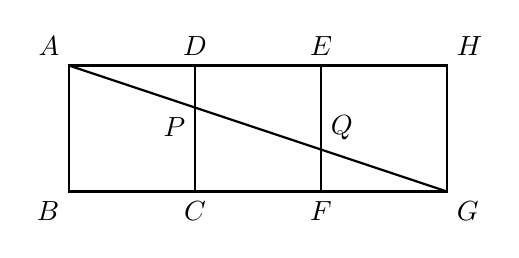
\begin{tikzpicture}[scale=0.8]
    \draw[thick] (0,0) rectangle (6,2);
    \draw[thick] (2,0) -- (2,2);
    \draw[thick] (4,0) -- (4,2);
    \draw[thick] (0,2) -- (6,0);
    \node[above left] at (0,2) {$A$};
    \node[below left] at (0,0) {$B$};
    \node[below] at (2,0) {$C$};
    \node[above] at (2,2) {$D$};
    \node[above] at (4,2) {$E$};
    \node[below] at (4,0) {$F$};
    \node[below right] at (6,0) {$G$};
    \node[above right] at (6,2) {$H$};
    \node[below left] at (2,1.33) {$P$};
    \node[above right] at (4,0.67) {$Q$};
\end{tikzpicture}
\end{minipage}
\begin{solution}
Since $\triangle ADP \sim \triangle AEQ \sim \triangle AHG$ with $AD : AE : AH = 1 : 2 : 3$, we have $\text{Area}(\triangle ADP) : \text{Area}(DEQP) = 1^2 : (2^2 - 1^2) = 1 : 3$. \\
Since $\text{Area}(\triangle AHG) = \frac{1}{2}\text{Area}(ABGH)$ and $\text{Area}(\triangle ADP) = \frac{1}{9}\text{Area}(\triangle AHG) = \frac{1}{6}\text{Area}(ABCD)$, we have $\text{Area}(ABCP) = 5 \times \text{Area}(\triangle ADP)$. \\
Thus, $\text{Area}(DEQP) : \text{Area}(ABCP) = 3 : 5$ (C).
\end{solution}